\section{Methode}\label{cha:method}

In diesem Kapitel wird die Spezialisierung eines \textit{CNN}s auf die Erkennung von Pilzbildern behandelt (siehe Kapitel \ref{cha:intr:aim}). Vorerst wird auf den Datenbeschaffungsprozess sowie der Datenvorverarbeitung eingegangen. Die darauf folgenden Abschnitte behandeln den Optimierungsprozess der \textit{Meta-Parameter} (siehe Kapitel \ref{cha:theo:backprop}, \ref{cha:theo:cnn} \& \ref{cha:theo:mod}) und erwähnen kurz diejenigen Massnahmen, welche zu einer signifikanten Verbesserung der Leistung des Erkennungsalgorithmus führten.

\subsection{Datenbeschaffung} \label{cha:met:datagathering}
Trainingsdaten bilden die Grundlage jedes auf \textit{Machine Learning} basierenden Algorithmus, weswegen man ein solides Fundament aus vielen Trainingsdaten benötigt (siehe Kapitel \ref{cha:theo:ml:training}). Da die Datenlage für Pilzbilder hingegen eher schlecht ist, ist die Datenbeschaffung ein wichtiger Bestandteil dieser Arbeit. Dabei gilt es, möglichst viele korrekt bestimmte Pilzbilder zu sammeln.

Für das Training sollen von jeder der 20 ausgewählten Pilzarten (siehe Tabelle \ref{table:shrooms}) mindestens 230 verschiedene Bilder beschaffen werden, von den unbekannten 1840 (das Achtfache). Um die Leistung des Algorithmus mittels unabhängigen Daten zu testen (siehe \textit{Validierung} in Kapitel \ref{cha:theo:ml:b-v}), werden zusätzlich 20 Bilder pro bekannte Art resp. 160 für die unbekannte Kategorie gesammelt. Somit mussten 250 Bilder pro ausgewählte Art sowie 2000 Bilder von unbekannten Arten gesammelt werden, insgesamt also etwa 7000 Bilder. Die Anzahl der bekannten Arten begründet sich mit den schwer verfügbaren Bilddaten, die der unbekannten durch eine erfahrungsgestützte Abschätzung, um im Rahmen einer Maturarbeit zu bleiben und trotzdem noch aussagekräftige Ergebnisse erhalten zu können.

Folgende Massnahmen wurden ergriffen, um möglichst viele, reine Trainingsdaten zu beschaffen:

\subsubsection{Datenbank SwissFungi}
Um einen Grunddatensatz zu erhalten, wurde die Fotodatenbank vom offiziellen SwissFungi Pilzatlas der WSL Schweiz verwendet\cite{wsl}. Von den 20 ausgewählten Arten konnten dadurch je einige Dutzend Bilder gesammelt werden; von den unbekannten Arten konnte die geforderte Anzahl von 2000 Exemplaren gedeckt werden. Diese Bilder sind alle professionell bestimmt und bedürfen daher keiner weiteren Kontrolle um die Datenreinheit zu garantieren. 

\subsubsection{Webseite ShroomNET}
Um Pilzsammler und Pilzfotografen aus der Region einfach zu erreichen, wurde die Webseite \textit{www.obermeier.ch} mit einem Hochladeformular für Pilzbilder eingerichtet. Aus einer Liste der ausgewählten Arten lässt sich die Kategorie auswählen, wobei die hochzuladenden Bilder mittels Drag-and-Drop direkt hochgeladen werden. Neben der Hochladefunktion wurde um die Datenreinheit zu gewährleisten zusätzlich ein \textit{Quiz} erstellt, bei dem Besucher die hochgeladenen Pilzbilder klassifizieren können. Mithilfe dieser Webseite lassen sich somit einfach weitere Bilder zusammentragen, welche auch direkt von erfahrenen Sammlern verifiziert werden können (siehe Abbildung \ref{img:webpage}).

Verbreitet wurde die Webseite über Telefonate und Mail-Verkehr mit Pilzkontrolleuren aus der Region Brugg-Aarau sowie in einem Artikel der Schweizerischen Zeitschrift für Pilzkunde SZP\cite{szp}, welche in der ganzen Schweiz versendet wurde. Mittels der Webseite konnten nochmals insgesamt etwa 300 Bilder gesammelt werden.

\subsubsection{Internet Crawler}
Mithilfe eines Python-Skriptes\cite{crawler} konnten automatisiert mit der Google-Suchmaschine nochmals etwa 400 Bilder pro Art gefunden und heruntergeladen werden, gesucht wurde dabei nach dem wissenschaftlichen Namen der Pilze. Aufgrund vieler Unreinheiten waren pro Kategorie nur etwa 150 weitere Bilder brauchbar. Da die Google-Suche nicht immer korrekte Ergebnisse liefert, wurden diese Bilder auf die Webseite hochgeladen, um sie im \textit{Quiz} nochmals von Pilzsammlern verifizieren zu lassen. 

\subsubsection{Videos}
Eine weitere Möglichkeit, um an viele Bilddaten zu kommen, ist das Extrahieren von Standbildern aus Videos. Bei sich ändernden Kameraperspektive lassen sich mehrere Standbilder von selben Pilz anfertigen, welche nicht identisch sind und sich daher als Trainingsdaten eignen. Dafür wurde das von Michael Bachmeier\cite{bachmeier} zur Verfügung gestellte Videomaterial verwendet. Insgesamt liessen sich durch die Bearbeitung von Videos weitere 1500 Bilder zur Datenbank hinzufügen. Auch diese Daten bedürfen aufgrund der zuverlässigen Quelle keiner weiteren Kontrolle.

\subsection{Datenaufbereitung}
Nach dem Sammeln der rohen Bilddaten gilt es in der Aufbereitung darum, die Bilder auf das Training anzupassen, d.h. Zentrieren sowie bildfüllendes Skalieren des Pilzes\footnote{Zwar könnten die Daten auch unbearbeitet in das Training eingespeist werden, jedoch erschwert die zusätzliche Lokalisierung des Pilzes den Lernprozess und führt unweigerlich zu einer Verschlechterung der Erkennungsleistung. Das Problem der Objektfindung in Bildern soll nicht Teil der Problemstellung sein, weswegen dieser Schritt hier manuell verrichtet wird.}. Dafür wurde eine Mindestauflösung von $200 \times 200$px festgelegt, welches eine gute Balance zwischen Details im Bild und Komplexität des Netzes bildet. Ein zu diesem Zwecke mit MatLab programmiertes Hilfsprogramm beschleunigte den manuellen Bearbeitungsprozess von Bildern wie auch Videos.
\begin{figure}[h]
	\centering
	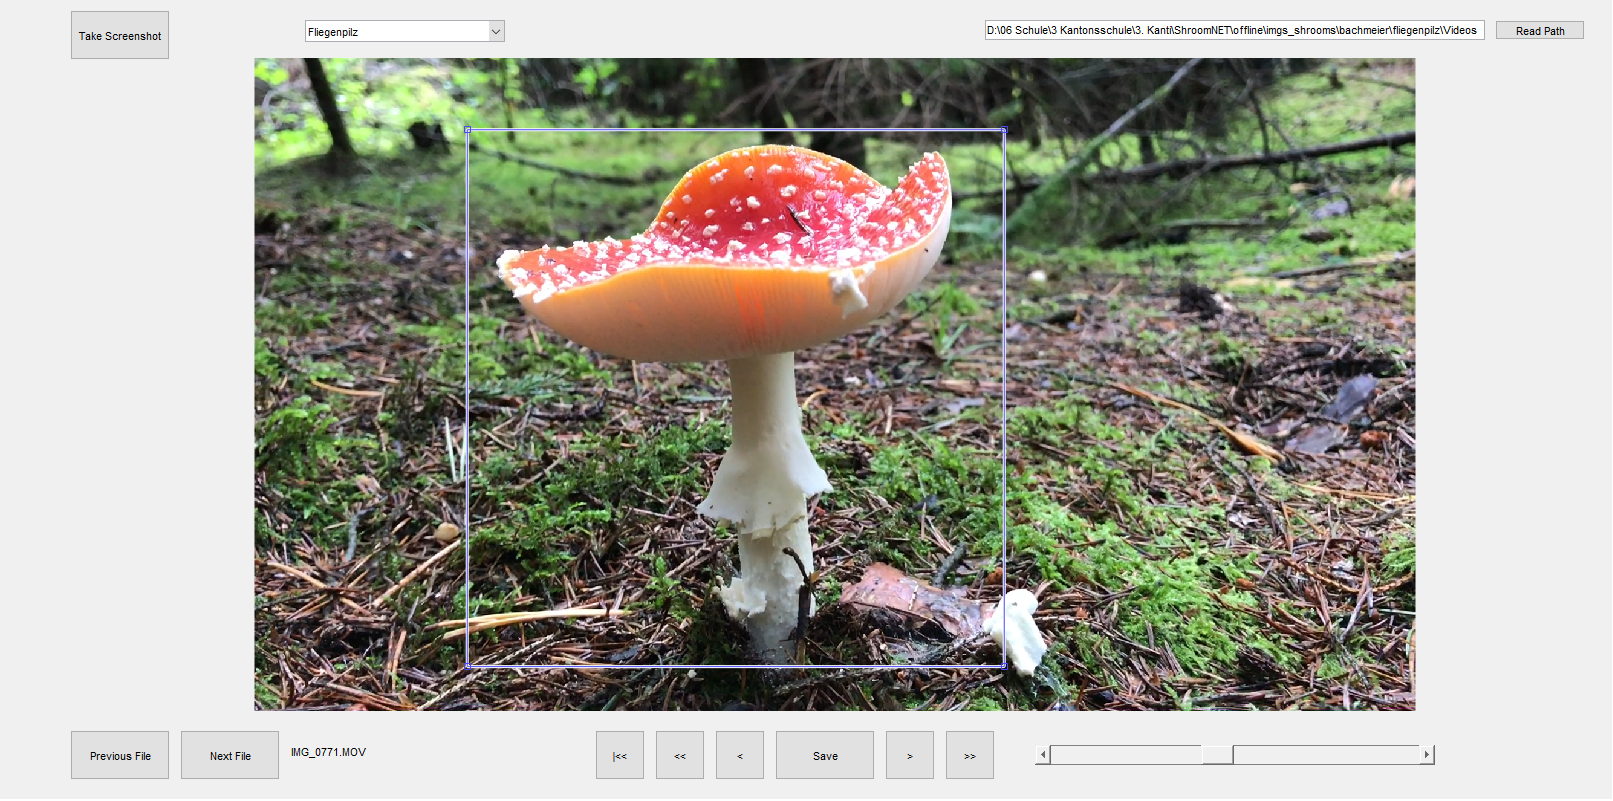
\includegraphics[width=\textwidth]{cropping}
	\caption[\textit{\textit{Hilfsprogramm}}]{Screenshot vom Hilfsprogramm beim Bearbeiten eines Videos: Oben links kann die Kategorie ausgewählt werden, der blaue Rahmen legt den Bildausschnitt fest. Unten befinden sich Steuerelemente zur Navigation sowie Speicherung des zugeschnittenen Bildes.}
	\label{img:precrocessing}
\end{figure}

Die zugeschnittenen Daten wurden in den vorher festgelegten Proportionen zufällig in Trainings- und Validierungsdaten unterteilt. Die aus Videos extrahierten Trainingsdaten eignen sich aufgrund der in Abbildung \ref{img:video_frames} ersichtlichen Ähnlichkeit nicht zur Validierung\footnote{Die Ähnlichkeit führte in ersten Tests zu einer Verfälschung der Ergebnisse.}, stattdessen werden diese ausschliesslich als Trainingsdaten verwendet.

\begin{figure}[h]
	\centering
	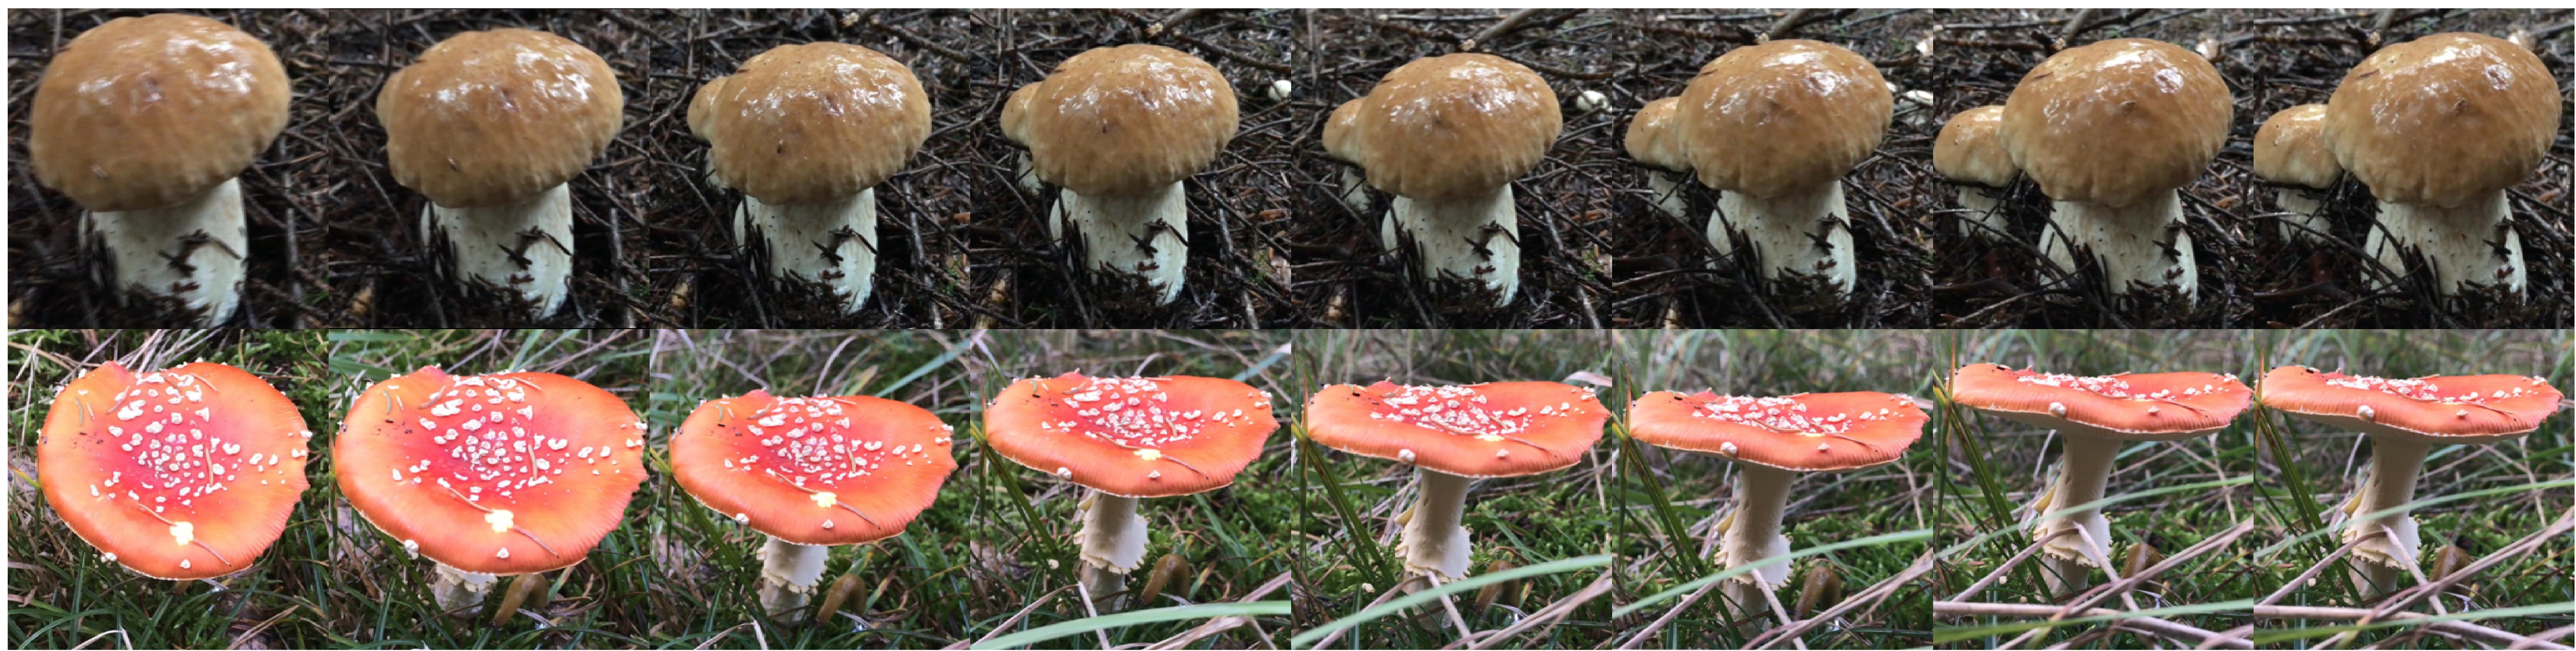
\includegraphics[width=\textwidth]{video_frames}
	\caption[\textit{\textit{Video-Frames}}]{8 Standbilder aus 2 Videos}
	\label{img:video_frames}
\end{figure}

Von gewissen Pilzarten waren weitaus mehr als 230 Bilder vorhanden. Dieser Überschuss musste ausgeglichen werden, damit von jeder Art gleich viele Trainingsbilder vorhanden sind. Statt diese überzähligen Exemplare aus dem Training auszuschliessen, wurden die Trainingsbilder mit Kopien zufälliger Exemplare der selben Kategorie auf 400 Bilder pro Pilzart ergänzt\footnote{Die Programmierumgebung von MatLab lässt keine benutzerdefinierte Verhältnisse der Kategorien zu, ohne tiefliegende Modifikationen an der \textit{Neural Network Library} vornehmen zu müssen. Daher diese Problemumgehung mittels Duplizieren einiger Trainingsdaten.}.

%Zusammengefasst ergeben sich aus der Datenbeschaffung und Datenaufbereitung folgende Zusammensetzung der Trainings- und Validierungsdaten:
%\begin{center}
%	\begin{tabular}{l | l | l | l | l}
%		Quelle & Training  & Training  & Validierung  & Validierung \\
%		  & bekannt & unbekannt & bekannt & unbekannt\\
%		\hline
%		SwissFungi & ca. 25 & 1840 & ca. 5 & 160\\
%		Webseite & ca. 15 & 0 & ca. 3 & 0\\
%		Crawler & ca. 130 & 0 & ca. 12 & 0\\
%		Video & ca. 75 & 0 & 0 & 0\\
%		\hline
%		\hline
%		& mind. 230
%	\end{tabular}
%\end{center}

\subsection{Entwicklungsprozess}\label{cha:met:dev}
Mit den aufbereiteten Trainingsdaten gilt es im nächsten Schritt den Algorithmus für die Pilzartenerkennung zu erarbeiten. In diesem Projekt wird hierfür die Entwicklungsumgebung MatLab mit der \textit{Deep Learning Toolbox} verwendet.

\subsubsection{Basis-SNN}

\subsubsection{Basis-CNN}

\subsubsection{Data-Augmentation}

\subsubsection{Farbfilter}

\subsubsection{Justierung des CNNs}

\subsubsection{Einspeisung von Zusatzinformationen}

\subsubsection{Transfer-Learning}

\subsubsection{CNN-Ensemble}